
\documentclass{article}
\usepackage{graphicx}
\usepackage{float}

\title{Hate Speech Detection}
\author{Vasile Godja}
\date{June 2024}

\begin{document}

\maketitle

\section{Introduction}
In today’s digital era, social media platforms influence public discourse. While they enable free expression, they also serve as breeding grounds for hate speech, which can lead to severe societal repercussions, including psychological harm, violence, and social discord. 

This raises the following question:
\begin{enumerate}
    \item \textbf{How effectively can various machine learning and deep learning models classify hate speech posts?}
\end{enumerate}

Our main goal is to find valuable insights and key metrics that can be used to train various models, which can be further incorporated into tools to prevent the spread of hate speech.
\section*{Data}

In order to answer these questions, we rely on the \textbf{hate\_speech18} dataset from Hugging Face's datasets library. This dataset contains text extracted from Stormfront, a white supremacist forum. A random set of forum posts has been sampled from several subforums and split into sentences. Those sentences have been manually labelled as containing hate speech or not, according to certain annotation guidelines \cite{gibert2018hate}.
An initial look at the dataset can be seen in Figure \ref{fig:first_rows}, which contains the columns text, user\_id, subforum\_id, num\_contexts, and label.

\begin{figure}[H]
    \centering
    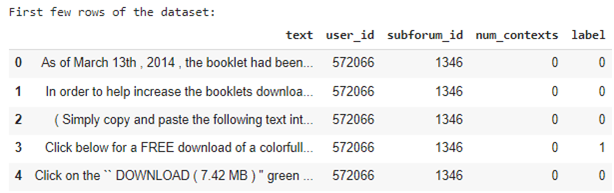
\includegraphics[width=\linewidth]{figure1.png}
    \caption{First few rows of the dataset}
    \label{fig:first_rows}
\end{figure}

The dataset has over 10,000 labeled social media posts. The distribution of labels is shown in Figure \ref{fig:label_distribution}, indicating that the majority of posts are classified as 0, while a smaller number are identified as 1, and even fewer as 2 and 3. The four labels present in the dataset are associated as follows:
\begin{enumerate}
    \item[0] Posts without hate speech or offensive content.
    \item[1] Posts explicitly promoting hate against individuals or groups.
    \item[2] Posts with unclear intent or insufficient context.
    \item[3] Posts that, when viewed in relation to others, may be considered hate speech.
\end{enumerate}


\begin{figure}[H]
    \centering
    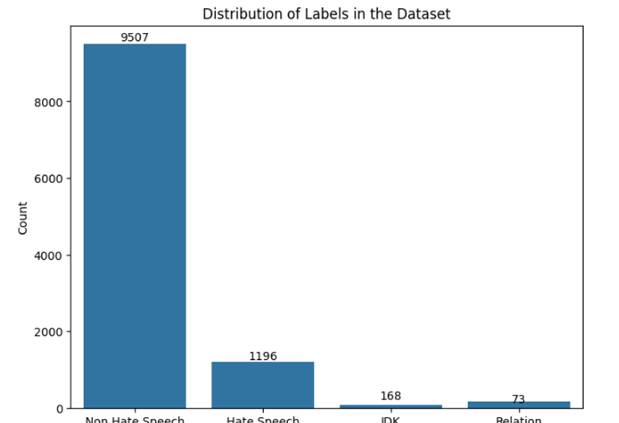
\includegraphics[width=\linewidth]{figure2.png}
    \caption{Distribution of Labels in the Dataset}
     \label{fig:label_distribution}
\end{figure}

\section*{Data Processing}

Prior to analysis and model training, we performed several preprocessing steps:

\begin{enumerate}
    \item Dropped unnecessary columns (user\_id, subforum\_id, num\_contexts).
    \item Filtered out labels 2 and 3 due to their representation of ambiguous content, which diverges from our main focus.
    \item Special Character Removal: Regular expressions were used to remove characters outside the alphanumeric range (a-z, A-Z); whitespace (\texttt{\textbackslash s}) and newline characters (\texttt{\textbackslash n}) were replaced with spaces.
    \item All text was converted to lowercase to ensure case-insensitive processing, avoiding treating "Good" and "good" as different words, simplifying the analysis.
    \item Stopword Removal: In order to reduce noise and emphasize content-carrying words, stopwords were removed using the Natural Language Toolkit (NLTK) library.
    \item Lemmatization: To capture the core meaning of words and improve model generalizability, we used lemmatization, which reduces words to their base form \cite{lemmatization}.
\end{enumerate}
Our preprocessing pipeline resulted in a dataset of 10,944 samples with an imbalanced class distribution, containing 1,196 samples labeled as hate speech and 9,507 labeled as non-hate speech (Figure \ref{fig:final_distribution}). This imbalance can hinder model training performance but can be addressed using oversampling or undersampling techniques.

\begin{figure}[H]
    \centering
    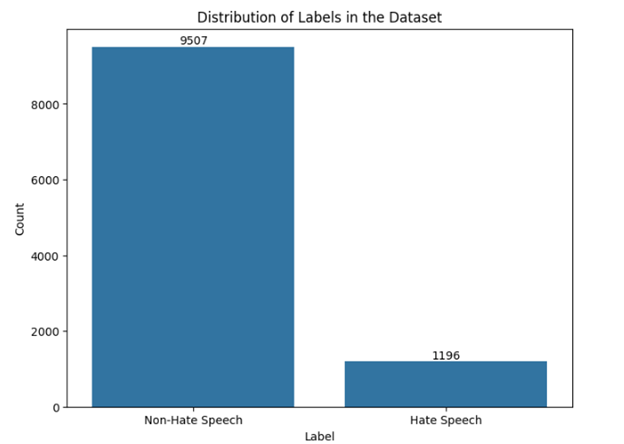
\includegraphics[width=\linewidth]{figure3.png}
    \caption{Final distribution of labels in the dataset}
    \label{fig:final_distribution}
\end{figure}

\section*{Results and Discussions}
\subsection*{LinearSVC }
Linear Support Vector Classifier is a powerful machine learning algorithm specifically designed for text classification tasks. It belongs to the family of support vector machines (SVMs), which are known for their ability to find optimal decision boundaries that separate data points into distinct classes \cite{scikit-learn}.


Our experiment employs pipelines, which are a convenient way to chain together data processing and model training steps. Each pipeline consists of three components:
\begin{enumerate}
    \item CountVectorizer: Converts textual data into a numerical representation by counting the occurrences of each word in the documents.
    \item TfidfTransformer: Considers both word frequency (TF) and inverse document frequency (IDF) to assign weights to words. Words that appear frequently across all documents receive lower weight, while those specific to hate speech documents gain higher weight, focusing on words that distinguish hate speech.
    \item Machine Learning Model: We evaluate three models:
        \begin{itemize}
            \item LinearSVC: A powerful algorithm for text classification that finds an optimal hyperplane to separate the data points (hate speech and non-hate speech) in the feature space created by TF-IDF.
            \item Random Forest: An ensemble method that combines multiple decision trees, improving model generalizability and reducing overfitting.
            \item Naive Bayes: A probabilistic classifier that assumes independence between features and calculates the probability of a document belonging to the hate speech class based on individual word probabilities.
        \end{itemize}
\end{enumerate}



\subsubsection{LinearSVC Performance}
Based on the results shown in Figure \ref{fig:model_performance}:
\begin{itemize}
    \item All models achieve relatively high accuracy scores (above 89\%), indicating their ability to classify hate speech and non-hate speech effectively.
    \item LinearSVC exhibits the best overall performance across most metrics. It achieves a balance between precision (correctly classifying hate speech) and recall (not missing true hate speech).
    \item Random Forest closely follows LinearSVC in accuracy but shows lower recall, suggesting it might miss some hate speech instances.
    \item Naive Bayes has the lowest performance, particularly in precision. While it seems to have a high recall, a significant portion might be false positives (incorrectly classifying non-hate speech as hate speech). This points towards potential overfitting and the need for further hyperparameter tuning for Naive Bayes.
\end{itemize}
\begin{figure}[H]
    \centering
    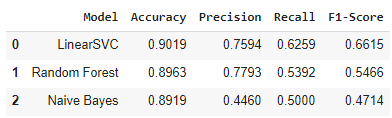
\includegraphics[width=\linewidth]{figure4.png}
    \caption{Model Performance Comparison}
    \label{fig:model_performance}
\end{figure}

\subsection*{SimpleRNN, LSTM, and Bidirectional SimpleRNN}
A recurrent neural network (RNN) is a type of artificial neural network which uses sequential data or time series data \cite{ibm-rnn}. In our case, we use some variants of RNNs:
\begin{enumerate}
    \item SimpleRNN: A basic RNN architecture that processes sequences one element (word) at a time. Each cell in a SimpleRNN takes the current input and the previous cell's output as inputs, allowing it to capture some short-term context within the sequence.
    \item LSTM (Long Short-Term Memory): A more sophisticated RNN architecture specifically designed to address the limitations of SimpleRNNs. LSTMs introduce memory cells with gates (input, output, forget) that control the flow of information:
        \begin{itemize}
            \item Input gate: Regulates the flow of new information into the cell.
            \item Output gate: Determines what information is passed on to the next cell.
            \item Forget gate: Controls what information from the previous cell is retained.
        \end{itemize}
\end{enumerate}

\subsubsection*{Neural Network Performance}
The performance evaluation of three neural network models—SimpleRNN, LSTM, and Bidirectional SimpleRNN—highlights the nuanced differences in handling sequential data tasks (Figure \ref{fig:nn_performance}). The LSTM model outperformed the others, achieving the highest accuracy (87.29\%), precision (65.58\%), recall (62.99\%), and F1-score (64.10\%). These metrics suggest its superior capability in managing long-term dependencies and minimizing both false positives and false negatives. The ROC-AUC score (62.99\%) further corroborates its proficiency in class discrimination. In contrast, the SimpleRNN model, with an accuracy of 86.55\% and lower precision and recall, indicates limitations in capturing complex patterns, likely due to the vanishing gradient problem. The Bidirectional SimpleRNN, while incorporating future context, showed a modest improvement over SimpleRNN but did not surpass the LSTM in overall performance. This comparison underscores the efficacy of LSTM architectures in applications requiring robust handling of sequential dependencies.

\begin{figure}[H]
    \centering
    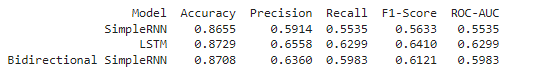
\includegraphics[width=\linewidth]{figure5.png}
    \caption{Neural Network Model Performance}
    \label{fig:nn_performance}
\end{figure}


\subsubsection*{DistilBERT}
DistilBERT is a pre-trained transformer model developed by Google AI \cite{distilbert}. It's a smaller and faster version of the original BERT model, making it ideal for tasks where computational resources are limited. Despite its reduced size, DistilBERT retains a significant amount of the language understanding capabilities of its larger counterpart.

Our experiment utilizes the transformers library to integrate DistilBERT into our hate speech detection pipeline. Here's a breakdown of the key steps:

\begin{enumerate}

    \item \textbf{Tokenization}: DistilBERT operates on sequences of tokens, which are smaller units of text (words or sub-words). We employ the DistilBertTokenizer class to convert our preprocessed text data into numerical token sequences.
    
    \item \textbf{Padding and Truncation}: Since DistilBERT requires sequences of a fixed length, we pad shorter sequences with special tokens and truncate longer sequences to ensure all input data conforms to the model's requirements.
    
    \item \textbf{Model Training}: The pre-trained DistilBERT model is fine-tuned on our labeled hate speech dataset. During fine-tuning, the model parameters are adjusted to specialize in classifying hate speech content.
    
    \item \textbf{Evaluation}: Once trained, the DistilBERT model is evaluated on a separate test dataset to assess its performance in generalizing to unseen hate speech examples. Metrics like accuracy, precision, recall, and F1-score are used to gauge the model's effectiveness.
\end{enumerate}
The DistilBERT model achieved an accuracy of 0.8828 on the training data during the final epoch. This indicates the model learned to classify hate speech content from the training examples. Furthermore, the evaluation on a separate test set yielded an accuracy of 0.8919 but we need to explore additional metrics beyond accuracy.

\subsubsection*{Conclusion}
Overall, the results demonstrate the potential of both traditional and deep learning models for hate speech detection. However, careful consideration of class imbalance and selection of appropriate metrics are necessary for robust evaluation. Our research partially answers the initial question by highlighting the effectiveness of various models. Further investigation into hyperparameter tuning and addressing class imbalance could lead to even better performance.

\bibliographystyle{plain}
\bibliography{references}

\end{document}